%%%%%%%%%%%%%%%%%%%%%%%%%%%%
% SECTION                  %
%%%%%%%%%%%%%%%%%%%%%%%%%%%%
\vspace{1em}

Un dilemme s'est posé lors de l'ajout des règles de MISP à celles des partenaires. Le nombre total de règles ingérées par les sondes se comptait auparavant en dizaine de milliers, mais une fois les règles MISP ajoutées, ce nombre s'élevait à des centaines de milliers.\\

\vspace{1em}

\begin{figure}[h]%
    \center%
    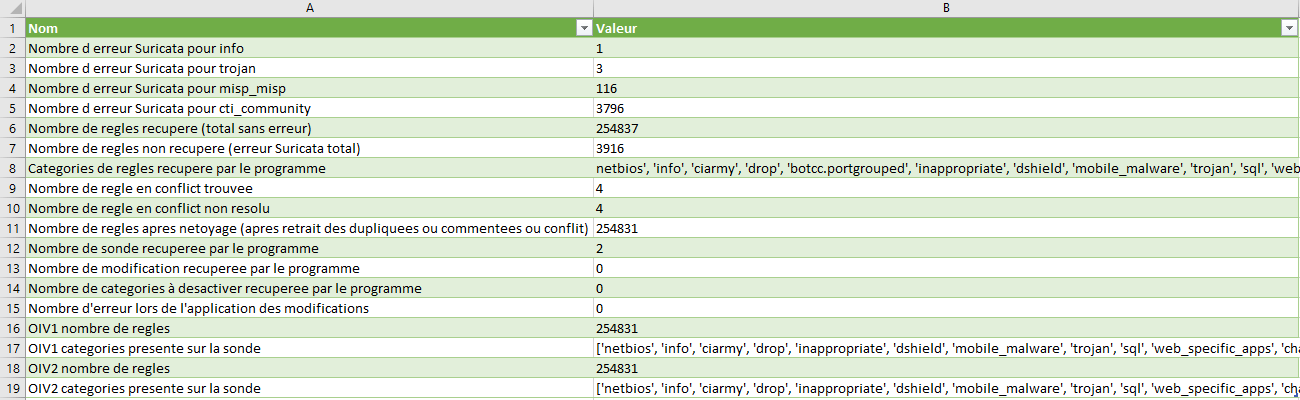
\includegraphics[width=1
    \textwidth]{assets/statMISP.png}
    \caption[Fichier CSV des statistique du programme après intégration des règles provenant de MISP]{Fichier CSV des statistique du programme après intégration des règles provenant de MISP}\label{fig:statMISP}
\end{figure}

\vspace{1em}

Ce nombre très élevé de règles risque de surcharger les sondes et de les ralentir, ce qui serait préjudiciable aux réseaux sur lesquels elles sont installées.\\

De plus, l'implémention de centaines de milliers de règles sans filtrage des sondes augmente considérablement le risque d'avoir des règles inutiles ou de provoquer de nombreux faux positifs (détection erronée d'une menace ou d'une activité malveillante par un système de sécurité) qui peuvent surcharger les équipes de sécurité de l'Agence. Un véritable défi se  pose alors pour filtrer les règles en fonction des OIV afin de maximiser leur efficacité et d'optimiser le nombre de règles appliquées à chaque sonde.\\

\newpage

 J'ai pu travailler sur ce point conjointement avec les membres du SOC-MC afin de hiérarchiser les règles en fonction de leur source et de leur type pour chaque OIV. D'une part, les règles fournies par les partenaires de renseignement sont classées en fonction de leur rôle et certaines d'entre elles sont destinées à des technologies spécifiques (par exemple 'SQL', 'ACTIVEX', 'SCADA', etc.). D'autre part dans l'environnement MISP, il est possible d'utiliser la fonctionnalité 'Tags' des événements pour trier les règles en catégories (par exemple les tags 'linux', 'windows', 'javascript', 'HealthCare', etc.).\\

En établissant ces catégories, nous pouvons ensuite, grâce à notre connaissance des technologies présentes sur les réseaux des OIV et leur collaboration avec l'Agence, estimer les règles pertinentes à retenir sur chaque sonde. Pour ce faire, j'ai complété \hyperref[chap3:section1]{\textbf{\textit{mon programme de gestion des règles}}} en ajoutant un segment permettant de désactiver des ensembles de règles en fonction de leur catégorie.\\

Ce nouveau segment fonctionne exactement comme \hyperref[chap3:section1rulesmodif]{\textbf{\textit{la section de modifications des règles}}}, mais utilise un autre fichier CSV fourni pour sélectionner les catégories de règles à supprimer pour les sondes.\\

\vspace{1em}

\begin{figure}[h]%
    \center%
    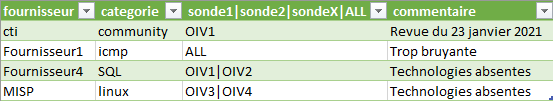
\includegraphics[width=0.8\textwidth]{assets/CategoriDisable.png}
    \caption[Exemple de fichier CSV de contrôle des catégories de règles]{Exemple de fichier CSV de contrôle des catégories de règles}\label{fig:CategoriDisable}
\end{figure}

\vspace{0.5em}

\begin{figure}[h]%
    \center%
\begin{lstlisting}[language=Python].
# Fonction pour parcourir les regles des sondes pour faire si possible la modification
def disable_categories(rulesByProbes, SelectedSondes, categorie, toDisable, modification_error):
    # On parcourt chaque sondes cible
    for sonde in SelectedSondes:
        # On cherche si la categorie existe dans la sonde cible
        if (categorie in rulesByProbes[sonde[0]]["source"].tolist()):
            targetRow = rulesByProbes[sonde[0]][rulesByProbes[sonde[0]]["source"].str.contains(categorie)]
            rulesByProbes[sonde[0]] = rulesByProbes[sonde[0]].drop(targetRow.index)
\end{lstlisting}
{\small
    \textit{Supprime les règles appartenant à certaines catégories sur des sondes ciblées.}
}
\caption[Contrôle des catégories sur les sondes]{Contrôle des catégories sur les sondes}\label{fig:RemoveCategorie}
\end{figure}

\newpage

Ce code ajouté permet de supprimer des milliers de règles ciblées sur chaque sonde, en ne conservant que celles qui sont les plus pertinentes, réduisant le nombre de règles par sonde à des niveaux plus supportables.

\vspace{1em}

\begin{figure}[h]%
    \center%
    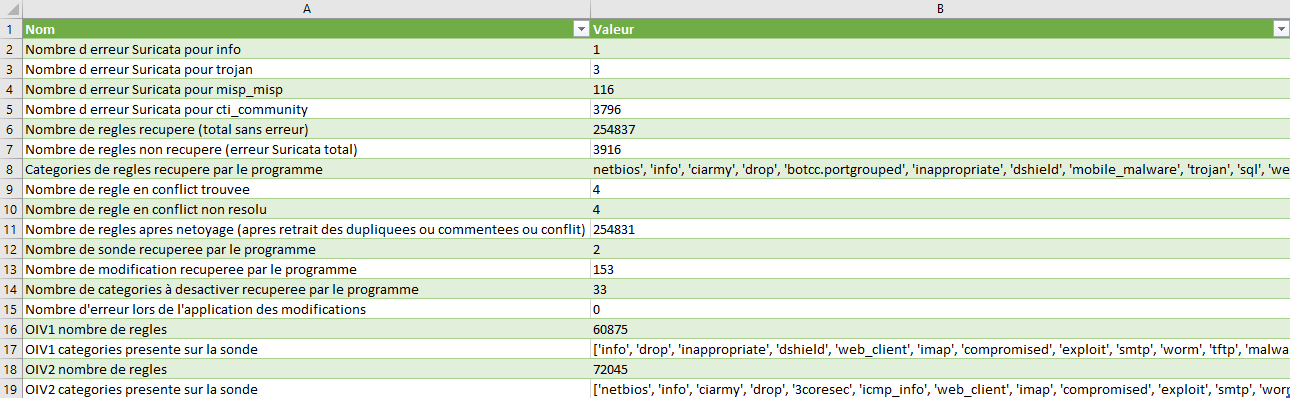
\includegraphics[width=1
    \textwidth]{assets/statOpti.png}
    \caption[Fichier CSV des statistiques du programme après sélection des catégories par sonde]{Fichier CSV des statistiques du programme après sélection des catégories par sonde}\label{fig:CategoriStat}
\end{figure}

\vspace{1em}

\subsubsection{\textit{Note}}
Cette partie s'est déroulée sur quelques semaines, incluant la complétion de la documentation réalisée précédemment avec les nouveaux changements. Ensuite, le temps restant de mon stage a été consacré à la rédaction de ma thèse professionnelle, à sa relecture et à sa correction en collaboration avec mon tuteur de stage.